\usetikzlibrary{arrows.meta}
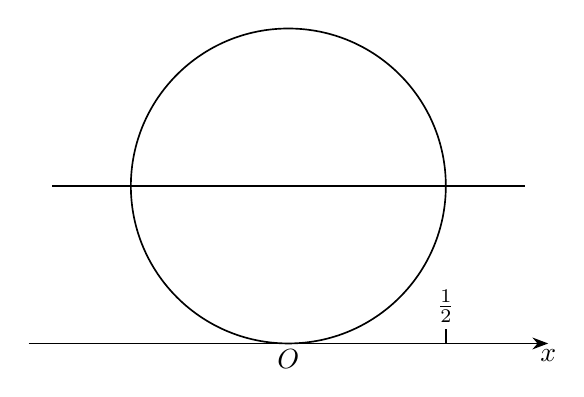
\begin{tikzpicture}[x=1cm,y=1cm,line width=.6pt,font=\normalsize,>=Stealth]
\draw[->] (-3.3,0)--(3.3,0);
\draw (-3.0,2.0)--(3.0,2.0);
\draw (0,2.0) circle[radius=2.0cm];
\draw[line width=.6pt] (2.0,0)--(2.0,0.18);
\node[anchor=north,inner sep=0pt,yshift=-2pt] at (0,0) {$O$};
\node[anchor=south,inner sep=0pt,yshift=2pt] at (2.0,0.18) {$\frac{1}{2}$};
\node[anchor=north,inner sep=0pt,yshift=-2pt] at (3.3,0) {$x$};
\end{tikzpicture}
